\section*{\nr.3 \titthree (10 Punkte)}
\begin{enumerate}[(a)]
\item Skizze siehe unten

\pgfplotsset{compat=newest}

\begin{figure}[htbp]
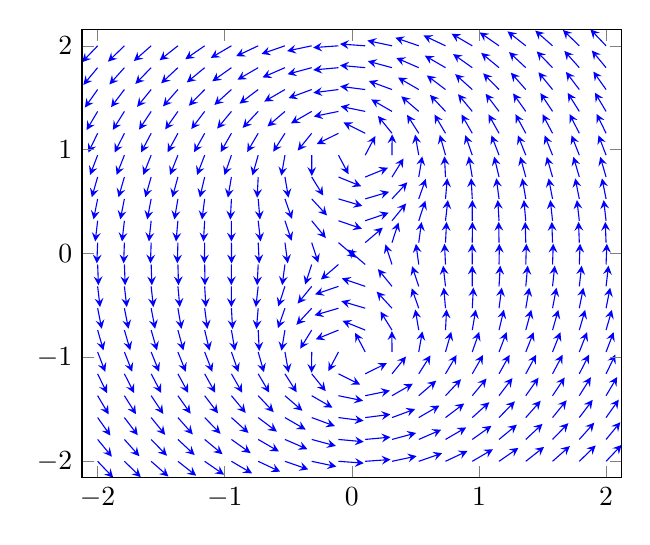
\begin{tikzpicture}
  \begin{axis}[
    domain=-2:2,
    view={0}{90},
    axis background/.style={fill=white},
  ]
    \addplot3[blue,
      quiver={
       u={(-(y+1)/(x^2+(y+1)^2)+(-y+1)/(x^2+(y-1)^2))/(sqrt((-(y+1)/(x^2+(y+1)^2)+(-y+1)/(x^2+(y-1)^2))^2+(x/(x^2+(y+1)^2)+(x)/(x^2+(y-1)^2))^2))},
       v={(x/(x^2+(y+1)^2)+(x)/(x^2+(y-1)^2))/(sqrt((-(y+1)/(x^2+(y+1)^2)+(-y+1)/(x^2+(y-1)^2))^2+(x/(x^2+(y+1)^2)+(x)/(x^2+(y-1)^2))^2))},
       scale arrows=0.2,
      },
      -stealth,samples=20]
        {1};
  \end{axis}
\end{tikzpicture}
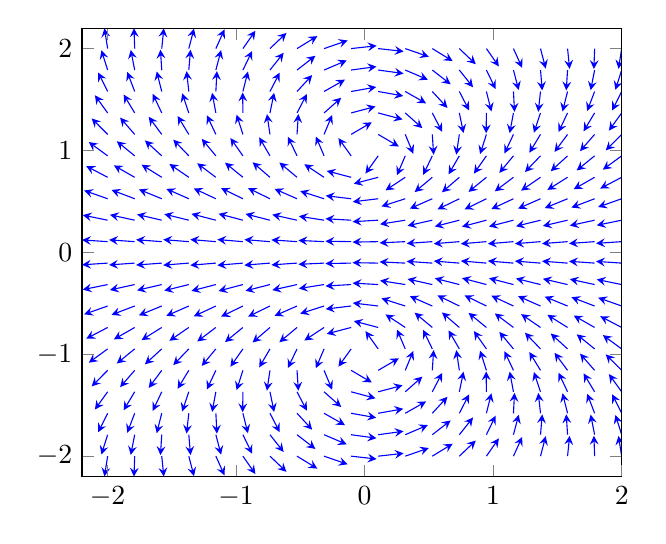
\begin{tikzpicture}
  \begin{axis}[
    domain=-2:2,
    view={0}{90},
    axis background/.style={fill=white},
  ]
    \addplot3[blue,
      quiver={
       u={(-(y+1)/(x^2+(y+1)^2)-(-y+1)/(x^2+(y-1)^2))/(sqrt((-(y+1)/(x^2+(y+1)^2)-(-y+1)/(x^2+(y-1)^2))^2+(x/(x^2+(y+1)^2)-(x)/(x^2+(y-1)^2))^2))},
       v={(x/(x^2+(y+1)^2)-(x)/(x^2+(y-1)^2))/(sqrt((-(y+1)/(x^2+(y+1)^2)-(-y+1)/(x^2+(y-1)^2))^2+(x/(x^2+(y+1)^2)-(x)/(x^2+(y-1)^2))^2))},
       scale arrows=0.2,
      },
      -stealth,samples=20]
        {1};
  ]
  \end{axis}
\end{tikzpicture}
\caption{\emph{Links:} Strom in gleicher Richtung, \emph{Rechts:} Strom in entgegengesetzter Richtung.}
\label{fig:same}
\end{figure}

\item Für das B-Feld gilt
\begin{equation}
  \vec B(x,y)=\frac{\mu_0}{2\pi}\left(\frac{1}{x^2+(y+a)^2}\begin{pmatrix}-y-a \\x\end{pmatrix}\pm \frac{1}{x^2+(y-a)^2}\begin{pmatrix}-y+a \\x\end{pmatrix}\right)
\end{equation}
wobei die beiden Terme bei Strom in gleicher Richtung addiert werden und bei Strom in entgegengesetzter Richtung subtrahiert.\\
Demnach gilt auf der x-Achse:
\begin{equation}
  \vec B(x,0)=\frac{\mu_0}{2\pi}\left(\frac{1}{x^2+a^2}\begin{pmatrix}-a \\x\end{pmatrix}\pm \frac{1}{x^2+a^2}\begin{pmatrix}a \\x\end{pmatrix}\right)\\
\end{equation}
Man erkennt insbesondere, dass für Strom in gleicher Richtung die x-Komponente, bei Strom in entgegengesetzter Richtung die y-Komponente gleich Null wird.
Für das B-Feld auf der y-Achse gilt
\begin{equation}
  \vec B(0,y)=\frac{\mu_0}{2\pi}\left(\frac{1}{(y+a)^2}\begin{pmatrix}-y-a \\0\end{pmatrix}\pm \frac{1}{(y-a)^2}\begin{pmatrix}-y+a \\0\end{pmatrix}\right)
\end{equation}
Man erkennt hier insbesondere, dass das Feld in y-Richtung immer gleich Null ist, egal in welche Richtung die Ströme fließen.

\item Da das Magnetfeld bei der gegebenen Konfiguration immer senkrecht auf dem Leiter steht gilt
\begin{equation}
  F_L=IlB
\end{equation}
mit $B=\frac{\mu_0}{4\pi a}$ folgt
\begin{equation}
  \frac{F_l}{l}=I^2 \frac{\mu_0}{4\pi a}=0.5\frac{\mathrm{mN}}{\mathrm{m}}
\end{equation}
Diese Kraft wirkt bei Strom in gleicher Richtung anziehend und bei Strom in entgegengesetzter Richtung abstoßend.

\item Die Kraft ist gleich Null, da das Magnetfeld und die Stromrichtung senkrecht aufeinander stehen, wordurch das Kreuzprodukt null wird.

\end{enumerate}